\documentclass[10pt]{jarticle}
\usepackage{float}
\usepackage{adrobo_abst}
\usepackage[dvipdfmx]{graphicx}
\usepackage{amssymb,amsmath}
\usepackage{bm}
\usepackage[superscript]{cite}
\usepackage{enumerate}
\usepackage{url}
%\usepackage[absolute]{textpos}

\renewcommand\citeform[1]{(#1)}

\begin{document}
    
    \makeatletter
    \doctype{2023年度卒業論文概要}
    \title{画像認識を用いた自動打刻の勤怠管理システム}{}
    \etitle{Attendance management system using image recognition}{}
    
    \author{19C1004\hspace{.5zw}池田泉海}
    \eauthor{Motomi Ikeda}
    
    \makeatother
    
    \abstract{We propose an automated the attendance management system.
    Conventional attendance management systems require manual time stamping.
    leading to problems such as the effort involved in stamping for each entry and exit,
    and the possibility of forgetting to stamp.
    To avoid this problem, we attempt to use image recognition to automate the time stamping process.
    The proposed method detects attendance and departure by employing image recognition to detect person.
    Automating the time stamping process has resulted in a reduction in effort for each entry and exit, and an improvement in the objectivity of the data.}
    
    \keywords{Attendance management system, Automated time stamping, Real-time object detection}
    
    \maketitle
    
    \supervisor{指導教員:上田隆一~准教授}
    
    \section{緒\hspace{2zw}言}%===========================
近年,労働環境の変化に伴い,効率的で正確な勤怠管理の重要性が増している.
そのため、勤怠管理システムでは,打刻に生態認証や顔認証を導入するなどして,
データの客観性が高められている.
しかし,ほとんどの勤怠管理システムは手動での打刻が必要であり,
手動打刻には出退勤毎の打刻労力や打刻忘れ等の問題が存在する.\par
本研究では,これらの問題に対処するためにYOLOv8\cite{Ultralitics2023}による画像認識で打刻を自動化した勤怠管理システムの提案を行う.
YOLOv8は物体検出アルゴリズムの一つで,
リアルタイムでの物体検出によく用いられている.
これはYOLOが画像を一度だけ見て物体の位置とクラスを同時に予測することで
高速な物体検出ができるためである.\par
これらの特徴を利用して,リアルタイムでカメラ画像から人物を検出することで打刻を自動化する.
打刻を自動化することで,従来の手動で打刻をする手法に比べ,利用者にとって手間を軽減し,打刻忘れを防止することができると考えられる.

    \section{構築するシステム}%===========================
本研究では、図\ref{configuration}に示した構成で勤怠管理システムを作成する。
システムの詳細について次項、次々項で説明する。

\begin{figure}[!h]
\centering
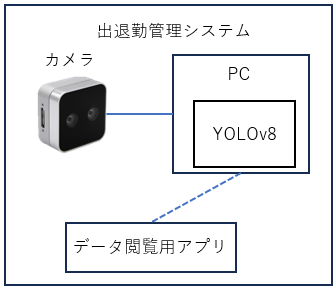
\includegraphics[width=0.7\linewidth]{fig/composition.png}
\caption{System configuration}
\label{configuration}
\end{figure}

    \subsection{入退室する人物の検出}
まず、部屋の出入り口にカメラを設置する。
設置したカメラは常時起動しておき映像を約0.2秒毎に画像で取得する。次に、取得した画像からYOLOv8を用いて人物を検出する。
人物が検出された場合、画像を保存する。
その日保存された画像のデータの最初と最後の画像を出勤時、退勤時とする。

    \subsection{出退勤時のデータをアプリにアップロード}
出退勤時の日時と画像データを担当者から閲覧可能にするため、
閲覧用のwebアプリを作成する。
作成したアプリにその日の画像データと日時データを、毎日決まった時間にアップロードする。


     
    \section{実験}%===========================
実際に動かしてるところを乗せる
マルバツで表を書く
何ができるのか
人物の認識
自動打刻


      
    \section{結\hspace{2zw}言}%===========================

    \vspace{1truemm}
    {\footnotesize
        \begin{thebibliography}{99}

            \bibitem{Ultralitics2023}
            Ultralytics (2023) ultralytics [Source code]. \url{https://github.com/ultralytics/ultralytics.}
        
        \end{thebibliography}
    }
    \normalsize
    
\end{document}
